\documentclass[11pt]{article}
\usepackage[margin=1in]{geometry}
\usepackage{amsmath,amssymb,mathtools}
\usepackage{amsthm}
\usepackage[american]{babel}
\usepackage{stmaryrd}
\usepackage{enumitem}
\usepackage{booktabs}
\usepackage{array}
\usepackage{listings}
\usepackage[x11names,table]{xcolor}
\usepackage{mdframed}
\usepackage{tikz}
\usepackage{url}
\usepackage[colorlinks=true,linkcolor=blue,citecolor=blue,urlcolor=blue]{hyperref}

\theoremstyle{plain}
\newtheorem{theorem}{Theorem}[section]
\newtheorem{proposition}[theorem]{Proposition}
\newtheorem{lemma}[theorem]{Lemma}
\newtheorem{corollary}[theorem]{Corollary}
\theoremstyle{definition}
\newtheorem{definition}[theorem]{Definition}
\theoremstyle{remark}
\newtheorem{remark}[theorem]{Remark}

\newcommand{\N}{\mathbb{N}}
\newcommand{\Z}{\mathbb{Z}}
\newcommand{\Q}{\mathbb{Q}}
\newcommand{\R}{\mathbb{R}}
\newcommand{\C}{\mathbb{C}}
\newcommand{\F}{\mathbb{F}}
\newcommand{\Fq}{\mathbb{F}_q}
\newcommand{\Qell}{\Q_\ell}
\newcommand{\Qlbar}{\overline{\Q}_\ell}
\newcommand{\A}{\mathbb{A}}
\newcommand{\calO}{\mathcal{O}}
\newcommand{\Gal}{\mathrm{Gal}}
\newcommand{\GL}{\mathrm{GL}}
\newcommand{\End}{\mathrm{End}}
\newcommand{\Frob}{\mathrm{Frob}}
\newcommand{\Tr}{\mathrm{Tr}}
\newcommand{\CRM}{\mathrm{CRM}}
\newcommand{\MaxSpec}{\mathrm{MaxSpec}}
\newcommand{\Cht}{\mathrm{Cht}}
\newcommand{\dualG}{\widehat{G}}

\newcommand{\BISH}{\mathsf{BISH}}
\newcommand{\LPO}{\mathsf{LPO}}
\newcommand{\WLPO}{\mathsf{WLPO}}
\newcommand{\LLPO}{\mathsf{LLPO}}
\newcommand{\MP}{\mathsf{MP}}
\newcommand{\FT}{\mathsf{FT}}
\newcommand{\CLASS}{\mathsf{CLASS}}

\definecolor{codegreen}{rgb}{0,0.6,0}
\definecolor{codegray}{rgb}{0.5,0.5,0.5}
\definecolor{codepurple}{rgb}{0.58,0,0.82}
\definecolor{backcolour}{rgb}{0.95,0.95,0.92}

\lstdefinelanguage{Lean}{
  keywords={theorem, lemma, def, definition, axiom, structure, class, instance,
            by, exact, intro, apply, have, show, fun, let, in,
            match, with, namespace, section, variable,
            import, open, noncomputable, classical,
            Type, Prop, forall, exists, where, extends,
            simp, decide, inductive, deriving, opaque, unfold, rw},
  sensitive=true,
  morecomment=[l]{--},
  morecomment=[s]{/-}{-/},
  morestring=[b]",
  literate=
    {→}{{$\rightarrow$}}1 {←}{{$\leftarrow$}}1
    {∀}{{$\forall$}}1 {∃}{{$\exists$}}1
    {∈}{{$\in$}}1 {≤}{{$\leq$}}1 {≥}{{$\geq$}}1
    {≠}{{$\neq$}}1 {∧}{{$\land$}}1 {∨}{{$\lor$}}1
    {¬}{{$\neg$}}1 {·}{{$\cdot$}}1
    {⟨}{{$\langle$}}1 {⟩}{{$\rangle$}}1
}

\lstdefinestyle{leanstyle}{
    language=Lean,
    backgroundcolor=\color{backcolour},
    commentstyle=\color{codegreen},
    keywordstyle=\color{blue},
    basicstyle=\ttfamily\footnotesize,
    breaklines=true,
    numbers=left,
    numbersep=5pt,
    numberstyle=\tiny\color{codegray}
}
\lstset{style=leanstyle}

\title{The Logical Cost of the Archimedean Place:\\
  Function Field Langlands is $\BISH$\\[6pt]
  {\large (Paper~69, Constructive Reverse Mathematics Series)}}

\author{Paul Chun-Kit Lee \\
New York University \\
\texttt{dr.paul.c.lee@gmail.com}}

\date{February 2026}

\begin{document}
\maketitle

\begin{abstract}
We perform a Constructive Reverse Mathematics ($\CRM$) audit of the function field
Langlands correspondence, classifying both Laurent Lafforgue's proof for $\GL_n$
(Inventiones, 2002) and Vincent Lafforgue's proof for general reductive groups
(JAMS, 2018). Both proofs are unconditionally $\BISH$: every component operates
within Bishop's constructive mathematics, with no omniscience principle required.

The classification itself is expected: the function field setting is algebraic
throughout. The paper's principal finding is the \emph{comparison} with number
fields. Paper~68 established that Wiles's proof route costs $\BISH + \WLPO$,
with the $\WLPO$ entering solely through the Arthur--Selberg trace formula at
the Archimedean place. The function field $\Fq(C)$ has no Archimedean place.
We show that every component which costs $\WLPO$ over number fields has an
algebraic counterpart over function fields that costs nothing: the
Grothendieck--Lefschetz trace formula replaces the Arthur--Selberg trace
formula; rational Plancherel measures replace transcendental ones;
finite-dimensional spaces of cusp forms replace infinite-dimensional $L^2$
spaces. The structural discovery underlying this comparison is that the
boundary between $\BISH$ and $\WLPO$ in the trace formula is not
discrete-vs-continuous spectrum, but algebraic-vs-transcendental spectral
parameters (\S\ref{sec:boundary}). The comparison yields:
\emph{the logical cost of the Langlands program is the logical cost of~$\R$}.

All results are formalized in Lean~4 (v4.28.0-rc1); the bundle compiles with
0~errors, 0~warnings, and 0~\texttt{sorry}s. No \texttt{Classical.choice}
appears in \texttt{\#print axioms} for any theorem.
\end{abstract}

\tableofcontents

% ============================================================
\section{Introduction}\label{sec:intro}
% ============================================================

\subsection{Main results}

The Langlands correspondence, in its function field incarnation, asserts a
bijection between cuspidal automorphic representations of $\GL_n(\A_F)$ (resp.\
$L$-packets for general reductive~$G$) and $n$-dimensional (resp.\
$\dualG$-valued) $\ell$-adic representations of $\Gal(\bar{F}/F)$, where
$F = \Fq(C)$ is the function field of a smooth projective curve over a finite
field. Two proofs are available: Laurent Lafforgue~\cite{LLaf02} for $\GL_n$
and Vincent Lafforgue~\cite{VLaf18} for general~$G$.

This paper applies Constructive Reverse Mathematics ($\CRM$) to both proofs
and establishes:

\begin{description}[leftmargin=2em]
\item[Theorem A] (Laurent Lafforgue, $\GL_n$). The five components of
  Laurent Lafforgue's proof---shtuka compactification, $\ell$-adic cohomology,
  Grothendieck--Lefschetz trace formula, function field Arthur--Selberg trace
  formula, and cuspidal isolation---each classify at~$\BISH$. The full proof
  is~$\BISH$.

\item[Theorem B] (Vincent Lafforgue, general~$G$). The five components of
  Vincent Lafforgue's proof---$G$-shtuka cohomology, geometric Satake
  equivalence, excursion operators, characters to Langlands parameters, and
  effective Chebotarev---each classify at~$\BISH$. The full proof is~$\BISH$.

\item[Theorem C] (Logical cost of $\R$). Every component of the Langlands
  program that costs $\WLPO$ over number fields (Paper~68~\cite{Paper68}) has a
  $\BISH$ counterpart over function fields. In each case, the structural source
  of the $\WLPO$ is traceable to the Archimedean place. This is a structural
  identification, not a proved lower bound (see \S\ref{sec:discussion} for
  discussion).
\end{description}

\noindent
The classification results (Theorems~A and~B) are expected: the function field
setting is algebraic, finite-dimensional, and defined over finite fields---any
competent constructivist would predict $\BISH$. The paper's principal
contribution is Theorem~C and the structural discovery underlying it
(\S\ref{sec:boundary}): the boundary between $\BISH$ and $\WLPO$ in the trace
formula is not discrete-vs-continuous spectrum but
algebraic-vs-transcendental spectral parameters. The Archimedean place makes
spectral parameters transcendental; removing it makes them algebraic. This is
the mechanism behind the thesis that the logical cost of the Langlands program
is the logical cost of~$\R$.

\subsection{Constructive Reverse Mathematics: a brief primer}

$\CRM$ calibrates mathematical statements against logical principles of
increasing strength within Bishop-style constructive mathematics ($\BISH$).
The hierarchy relevant to this paper is:
\[
\BISH \;\subset\; \BISH + \WLPO \;\subset\; \BISH + \LPO
  \;\subset\; \CLASS.
\]
(The full lattice also includes $\MP$ and $\LLPO$, which are independent of
each other over $\BISH$; they do not appear in this paper.)
Here $\WLPO$ (Weak Limited Principle of Omniscience) states that for every
binary sequence~$\alpha$, either $\alpha = 0^\omega$ or
$\lnot(\alpha = 0^\omega)$. Equivalently, for every real~$x$, either $x = 0$
or $\lnot(x = 0)$. For a thorough treatment of $\CRM$, see
Bridges--Richman~\cite{BridgesRichman1987}; for the broader program of which
this paper is part, see Papers~1--68 of this series and the atlas
survey~\cite{Paper50}.

\subsection{Current state of the art}

The function field Langlands correspondence for $\GL_n$ was proved by
Drinfeld~\cite{Drinfeld80} ($n = 2$) and Laurent Lafforgue~\cite{LLaf02}
(general~$n$). The automorphic-to-Galois direction for general reductive~$G$
was proved by Vincent Lafforgue~\cite{VLaf18}. No prior work has applied
$\CRM$ to the logical structure of these proofs.

Over number fields, Paper~68~\cite{Paper68} audited Wiles's proof of Fermat's
Last Theorem, establishing $\CRM(\text{FLT}) = \BISH$ while showing that
Wiles's 1995 proof route costs $\BISH + \WLPO$. The $\WLPO$ entered through
the Langlands--Tunnell theorem at weight~1, which uses the Arthur--Selberg
trace formula at the Archimedean place. Paper~68, \S13 posed the question:
is the $\WLPO$ intrinsic to the Langlands program, or is it an artifact of the
Archimedean place?

\subsection{Position in the atlas}

This is Paper~69, the final audit paper of the $\CRM$ series (Paper~70
provides the synthesis). The series began with Papers~2 and~7 (Banach space
non-reflexivity at~$\WLPO$), progressed through Paper~6 (Heisenberg
uncertainty), Paper~8 (Ising model and $\LPO$), Paper~45 (Weight-Monodromy
Conjecture and de-omniscientizing descent), Papers~50--53 (atlas survey and DPT
framework~\cite{Paper50,Paper53}), and Paper~68 (Fermat's Last Theorem). The
present paper resolves the open question from Paper~68: the $\WLPO$ is not
intrinsic to the Langlands program. It enters through the Archimedean place and
vanishes upon removing it. Paper~70~\cite{Paper70} synthesizes the full series.

The de-omniscientizing descent pattern (Paper~45~\cite{Paper45}) identified
geometric origin as a decidability descent mechanism: motives with geometric
origin have their logical cost reduced from $\LPO$ to $\BISH$. Removing the
Archimedean place is the proof-methods analogue: it eliminates the
transcendental content that generates omniscience requirements. Both are
instances of the same structural phenomenon---descent from a higher omniscience
principle to $\BISH$ upon imposing an algebraicity constraint.

% ============================================================
\section{Preliminaries}\label{sec:prelim}
% ============================================================

\begin{definition}[Weak Limited Principle of Omniscience]
$\WLPO$ is the assertion that for every binary sequence $a : \N \to \{0,1\}$,
either $\forall n,\; a(n) = 0$ or $\lnot(\forall n,\; a(n) = 0)$.
\end{definition}

\begin{definition}[Function field]
Let $C/\Fq$ be a smooth projective geometrically connected curve with function
field $F = \Fq(C)$. Each closed point $v \in |C|$ gives a local field
$F_v \cong k_v((t))$. Every local field is non-Archimedean. There is no real
or complex place, no continuous characters on $i\R$, no Gamma factors.
\end{definition}

\begin{definition}[Shtuka]
A shtuka of rank~$r$ over an $\Fq$-scheme $S$ with legs $x_i : S \to C$ is a
vector bundle $\mathcal{E}$ on $C \times S$ equipped with a modification of its
Frobenius pullback, with poles and zeros along the graphs of the~$x_i$. The
moduli stack $\Cht_{r,I}$ is a Deligne--Mumford stack over~$C^I$.
\end{definition}

\begin{definition}[CRM join]
For a proof depending on components $c_1, \ldots, c_k$ with CRM levels
$\ell_1, \ldots, \ell_k$, the CRM level of the proof is
$\ell_1 \vee \cdots \vee \ell_k$ (the supremum in the CRM lattice).
\end{definition}

\noindent
The logical principles used in this paper ($\BISH$, $\WLPO$) are defined
precisely in Bridges--Richman~\cite{BridgesRichman1987}. All proofs in this
section are deferred to~\S\ref{sec:main}.

% ============================================================
\section{Main Results}\label{sec:main}
% ============================================================

\subsection{Laurent Lafforgue's proof for $\GL_n$ (Theorem~A)}

We audit five components of~\cite{LLaf02,Rapoport02,Laumon00}.

\begin{proposition}[Compactification of shtuka moduli]\label{prop:compact}
The compactification of $\Cht_{r,N}$ is $\BISH$.
\end{proposition}

\begin{proof}
Lafforgue's compactification uses iterated blow-ups along boundary strata
classified by Harder--Narasimhan types. All constructions are explicit algebraic
intersection theory on Deligne--Mumford stacks over~$\Fq$. No Archimedean
topology, no transcendental analysis, no omniscience principle.
\end{proof}

\begin{proposition}[$\ell$-adic cohomology]\label{prop:etale}
The \'etale cohomology of shtuka stacks is $\BISH$.
\end{proposition}

\begin{proof}
The groups $H^i_c(\Cht_{r,N} \otimes \overline{\Fq}, \Qell)$ are
finite-dimensional $\Qell$-vector spaces, with Frobenius eigenvalues that are
algebraic numbers (Weil numbers) by Deligne's purity theorem~\cite{Deligne80}.

\emph{Foundational caveat.} The cohomological machinery---derived categories,
proper base change, Poincar\'e duality---is developed over~$\Fq$ in
SGA~4/4$\tfrac{1}{2}$. The standard treatment of derived categories uses Zorn's
lemma for injective resolutions, and the existence of enough injectives in
sheaf categories relies on classical set-theoretic machinery. The $\BISH$
classification applies not to this foundational setup but to the
\emph{computational content extracted from the proof}: once the cohomology
groups are established as finite-dimensional $\Qell$-vector spaces with
algebraic Frobenius eigenvalues, all subsequent operations---computing traces,
comparing eigenvalues, testing equalities---are decidable finite linear algebra.
This distinction between ``proof route'' (potentially classical foundational
machinery) and ``intrinsic cost'' (the computational content of the result) is
the same one employed in Paper~68~\cite{Paper68}, \S4 for commutative algebra
over Noetherian rings.
\end{proof}

\begin{proposition}[Grothendieck--Lefschetz trace formula]\label{prop:GL-trace}
The Grothendieck--Lefschetz trace formula is $\BISH$.
\end{proposition}

\begin{proof}
The formula $\#\Cht_{r,N}(\Fq) = \sum_i (-1)^i \Tr(\Frob_q \mid H^i_c)$
evaluates as a finite sum of algebraic numbers on finite-dimensional vector
spaces. Equality of algebraic numbers is decidable: elements of $\overline{\Q}$
are roots of polynomials with rational coefficients, and coincidence is
decided by root isolation (quantifier elimination for algebraically closed
fields).
\end{proof}

\begin{proposition}[Function field Arthur--Selberg trace formula]\label{prop:AS-func}
The function field Arthur--Selberg trace formula is $\BISH$.
\end{proposition}

\begin{proof}
Laurent Lafforgue compares the Grothendieck--Lefschetz geometric side with the
Arthur--Selberg spectral side. The quotient
$\GL_r(F) \backslash \GL_r(\A_F)$ is \emph{not} compact modulo centre: cusps
exist. Continuous spectrum and Eisenstein series are present.

However, the local fields $F_v = k_v((t))$ are totally disconnected. Unramified
characters of $F_v^\times$ are parametrized by $z = q_v^{-s}$ on a compact
algebraic torus $(\C^\times)^{r-1}$, not on~$i\R$. The intertwining operators
$M(s,\pi)$ and their normalizing factors (local $L$-functions) are rational
functions of $q^{-s}$ (Langlands~\cite{Langlands71}; see~\cite{Laumon00},
\S3 for the function field case). The Plancherel measure is a rational function
of these same variables. Eisenstein series are rational in~$z$.

The spectral contribution of the continuous spectrum is therefore a contour
integral of a rational function over a compact algebraic torus. By the residue
theorem (applied to rational functions on $\C^\times$---a finite algebraic
computation, not a transcendental one), this reduces to a finite sum of
algebraic residues. Arthur's truncation operators, which in the number field
setting involve real-valued truncation parameters, are here applied to rational
functions of~$q^{-s}$; the truncated sums remain algebraic.
\end{proof}

\subsection{The algebraic-vs-transcendental boundary}\label{sec:boundary}

The result of Proposition~\ref{prop:AS-func} is the principal surprise of the
audit. To appreciate why, we must explain the na\"ive expectation, show why it
is wrong, and identify the correct boundary.

\medskip\noindent
\textbf{The na\"ive expectation.}
The trace formula (Arthur--Selberg or Grothendieck--Lefschetz) has a spectral
side and a geometric side. The spectral side decomposes the automorphic
representation space into irreducible components. When the spectrum is
\emph{discrete}---a countable list of eigenvalues---the spectral side is a
sum. Each term is an algebraic number (a Frobenius eigenvalue or Hecke
eigenvalue), and finite sums of algebraic numbers are decidable. This is
$\BISH$. When the spectrum is \emph{continuous}---the quotient
$G(F) \backslash G(\A_F)$ is not compact, and Eisenstein series span a
continuous family---the spectral side involves an integral over a continuum of
spectral parameters. Testing whether two real-valued integrals are equal
requires testing exact real equality: $\WLPO$. The na\"ive expectation is
therefore:
\[
\text{discrete spectrum} \;\Rightarrow\; \BISH, \qquad
\text{continuous spectrum} \;\Rightarrow\; \WLPO.
\]

\medskip\noindent
\textbf{Why the na\"ive expectation is wrong.}
Over function fields, continuous spectrum \emph{exists}. For $\GL_r$ with
$r \ge 2$, the quotient $\GL_r(F) \backslash \GL_r(\A_F)$ is not compact
modulo centre: there are cusps, and Eisenstein series span a non-trivial
continuous family. If the na\"ive expectation were correct, the function field
trace formula would cost $\WLPO$. It does not.

The reason is that the spectral parameters over function fields are
\emph{algebraic}. Unramified characters of the local group $\GL_1(F_v)$ for
$F_v = k_v((t))$ are parametrized by $z = q_v^{-s}$, a coordinate on the
multiplicative group $\C^\times$. For $\GL_r$, the continuous spectrum lives on
the compact torus $|z_1| = \cdots = |z_{r-1}| = 1$ inside
$(\C^\times)^{r-1}$. The intertwining operators $M(s,\pi)$, their normalizing
$L$-factors, and the Plancherel measure are all \emph{rational functions}
of~$z$ (Langlands~\cite{Langlands71}; \cite{Laumon00}, \S3). The Eisenstein
series themselves are rational in~$z$.

The spectral contribution of the continuous spectrum is therefore a contour
integral of a rational function over an algebraic torus. A contour integral of
a rational function computes by the residue theorem: finitely many poles,
each with an algebraic residue, yielding a finite sum of algebraic numbers.
This is a finite algebraic operation---not a transcendental one. The continuous
spectrum contributes a decidable quantity. That is $\BISH$.

\medskip\noindent
\textbf{The contrast with number fields.}
Over number fields, the same structural decomposition applies---the spectrum
has a discrete part and a continuous part, and the continuous part is handled
by Eisenstein series. But the spectral parameters are now transcendental. The
Archimedean local field~$\R$ contributes characters $|\cdot|^s$ with
$s \in i\R$. The intertwining operators involve the Gamma function
$\Gamma(s)$---a transcendental function of a transcendental variable.
The Plancherel measure involves $|\Gamma(s)|^2$. The spectral contribution
of the continuous spectrum is an integral of a transcendental function
over~$\R$, not a contour integral of a rational function over an algebraic
torus. The residue theorem does not reduce this to a finite algebraic sum.

Deciding whether two such integrals are equal---or whether a particular
eigenvalue is embedded in the continuous spectrum---requires testing exact
equality of real numbers. That is $\WLPO$. The Archimedean place makes the
spectral parameters transcendental, and transcendence is what forces the
logical cost.

\medskip\noindent
\textbf{The correct boundary.}
The logical cost comes from the \emph{nature} of the spectral parameters
(algebraic vs.\ transcendental), not from the \emph{topology} of the spectrum
(discrete vs.\ continuous). One can have continuous spectrum that is logically
free---as over function fields, where the parameters are algebraic and
the integral computes by residues. Conversely, one could in principle have
discrete spectrum that is logically expensive, if the eigenvalues were
transcendental numbers whose equality was undecidable in $\BISH$.

The Archimedean place makes spectral parameters transcendental. That---not
continuity of the spectrum---is what triggers $\WLPO$. Removing the
Archimedean place (passing from~$\Q$ to~$\Fq(C)$) replaces transcendental
parameters with algebraic ones. The continuous spectrum remains, but its
logical cost vanishes. Figure~\ref{fig:boundary} summarizes the situation.

\begin{figure}[ht]
\centering
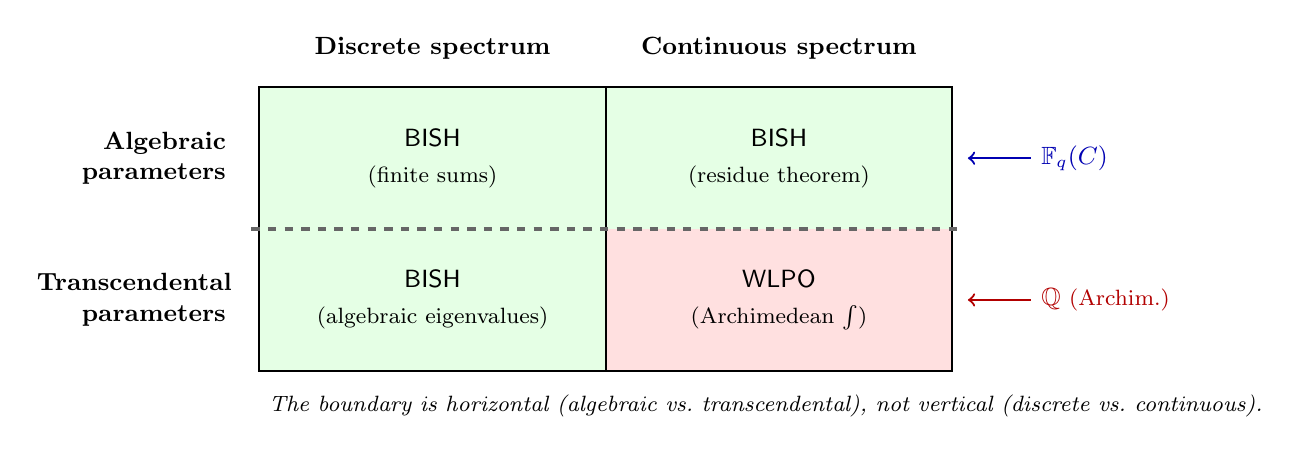
\begin{tikzpicture}[
  cell/.style={minimum width=4.4cm, minimum height=1.8cm, align=center,
               font=\small},
  header/.style={font=\small\bfseries, align=center},
  rowlabel/.style={font=\small\bfseries, align=right, anchor=east,
                   text width=2.4cm},
]

% Shading (drawn first, behind everything)
\fill[green!10] (0,1.8) rectangle (8.8,3.6);
\fill[green!10] (0,0) rectangle (4.4,1.8);
\fill[red!12] (4.4,0) rectangle (8.8,1.8);

% Grid
\draw[thick] (0,0) rectangle (8.8,3.6);
\draw[thick] (4.4,0) -- (4.4,3.6);
\draw[ultra thick, dashed, black!60] (-0.1,1.8) -- (8.9,1.8);

% Column headers
\node[header] at (2.2,4.1) {Discrete spectrum};
\node[header] at (6.6,4.1) {Continuous spectrum};

% Row labels (horizontal, to the left)
\node[rowlabel] at (-0.3,2.7) {Algebraic\\parameters};
\node[rowlabel] at (-0.3,0.9) {Transcendental\\parameters};

% Cell contents
\node[cell] at (2.2,2.7) {$\BISH$\\[2pt]{\footnotesize (finite sums)}};
\node[cell] at (6.6,2.7) {$\BISH$\\[2pt]{\footnotesize (residue theorem)}};
\node[cell] at (2.2,0.9) {$\BISH$\\[2pt]{\footnotesize (algebraic eigenvalues)}};
\node[cell] at (6.6,0.9) {$\WLPO$\\[2pt]{\footnotesize (Archimedean $\int$)}};

% Right-side annotations
\draw[->, thick, blue!70!black]
  (9.8,2.7) node[right, font=\small, text=blue!70!black] {$\Fq(C)$}
  -- (9.0,2.7);
\draw[->, thick, red!70!black]
  (9.8,0.9) node[right, font=\small, text=red!70!black]
  {$\Q$ \footnotesize{(Archim.)}} -- (9.0,0.9);

% Bottom annotation
\node[font=\footnotesize\itshape, anchor=west] at (0,-0.45)
  {The boundary is horizontal (algebraic vs.\ transcendental),
   not vertical (discrete vs.\ continuous).};

\end{tikzpicture}
\caption{The CRM boundary in the trace formula. Function fields
  ($\Fq(C)$, top row) have algebraic spectral parameters: both discrete
  and continuous spectrum are $\BISH$. Number fields ($\Q$, bottom-right)
  have transcendental spectral parameters at the Archimedean place,
  forcing $\WLPO$. The dashed line marks the true boundary.}
\label{fig:boundary}
\end{figure}

\begin{proposition}[Cuspidal isolation]\label{prop:isolation}
Isolation of the cuspidal component is $\BISH$.
\end{proposition}

\begin{proof}
By Harder's theorem~\cite{Harder74}, the space of cusp forms
$C_{\mathrm{cusp}}(\GL_r(F) \backslash \GL_r(\A_F) / K)$ is
finite-dimensional. Decomposition into $\pi$-isotypic components is finite
linear algebra. Over number fields, the analogous space at weight~1 has no
algebraic dimension formula (Paper~68, \S11.4). Over function fields, there is
no weight, and Harder's theorem provides finiteness unconditionally.
\end{proof}

\begin{theorem}[Theorem~A]\label{thm:Laurent-main}
$\CRM(\text{Laurent Lafforgue, } \GL_n/\Fq(C)) = \BISH$.
\end{theorem}

\begin{proof}
The join of the five component levels
(Propositions~\ref{prop:compact}--\ref{prop:isolation}) is
$\BISH \vee \BISH \vee \BISH \vee \BISH \vee \BISH = \BISH$.
\end{proof}

\subsection{Vincent Lafforgue's proof for general $G$ (Theorem~B)}

Vincent Lafforgue~\cite{VLaf18,VLafICM} proves the automorphic-to-Galois
direction for split reductive $G/\Fq(C)$, explicitly independent of the
Arthur--Selberg trace formula.

\begin{proposition}[$G$-shtuka cohomology and geometric Satake]\label{prop:Satake}
$G$-shtuka cohomology and the geometric Satake equivalence are $\BISH$.
\end{proposition}

\begin{proof}
The moduli stacks $\Cht_I$ are Deligne--Mumford stacks over $C^I$, with
finite-dimensional $\ell$-adic cohomology. The geometric Satake
equivalence~\cite{MV07}---a tensor equivalence between perverse sheaves on
the affine Grassmannian and representations of $\dualG$---is constructed via
intersection cohomology of affine Schubert varieties over~$\Fq$.
The BBD decomposition theorem (Beilinson--Bernstein--Deligne~\cite{BBD82})
underlies the semisimplicity of the relevant categories. Over~$\Fq$ with
$\Qlbar$-coefficients, semisimplicity follows from Deligne's purity:
Frobenius eigenvalues are computable algebraic numbers (Weil numbers), and
the weight filtration splits by algebraic linear algebra. The perverse
$t$-structure is defined by combinatorial support/cosupport conditions.
All constructions are algebraic.
\end{proof}

\begin{proposition}[Excursion operators]\label{prop:excursion}
The excursion algebra and its spectral decomposition are $\BISH$.
\end{proposition}

\begin{proof}
From shtuka cohomology and geometric Satake, Vincent Lafforgue constructs
excursion operators
$S_{I,f,(\gamma_i)} \in \End_{\Qlbar}(C_{\mathrm{cusp}}(K))$ generating a
commutative $\Qlbar$-algebra~$B$. Since $C_{\mathrm{cusp}}(K)$ is
finite-dimensional (Harder~\cite{Harder74}), the image of $B$ in
$\End(C_{\mathrm{cusp}}(K))$ is a finite-dimensional commutative
$\Qlbar$-algebra, hence Artinian. Its $\MaxSpec$ is finite and computable by
simultaneous triangularization.
\end{proof}

\begin{proposition}[Characters to Langlands parameters]\label{prop:chars}
Characters to Langlands parameters and effective Chebotarev are $\BISH$.
\end{proposition}

\begin{proof}
Each character $\nu : B \to \Qlbar$ determines Frobenius traces at every
place. By pseudo-character theory
(Taylor~\cite{Taylor91}, Rouquier~\cite{Rouquier96}) and Chevalley's
restriction theorem, a semisimple conjugacy class in $\dualG$ is uniquely
determined by polynomial evaluations on fundamental representations. Effective
Chebotarev over function fields (from the Weil conjectures~\cite{Weil48},
giving polynomial bounds) ensures bounded searches.
\end{proof}

\begin{theorem}[Theorem~B]\label{thm:Vincent-main}
$\CRM(\text{Vincent Lafforgue, general } G/\Fq(C)) = \BISH$.
\end{theorem}

\begin{proof}
The five components ($G$-shtuka cohomology, geometric Satake, excursion
algebra, characters to parameters, effective Chebotarev) are audited in
Propositions~\ref{prop:Satake}--\ref{prop:chars}, each classified at~$\BISH$.
The join is $\BISH \vee \BISH \vee \BISH \vee \BISH \vee \BISH = \BISH$.
\end{proof}

\subsection{The logical cost of $\R$ (Theorem~C)}

\begin{table}[ht]
\centering
\caption{CRM comparison: number field vs.\ function field Langlands.}
\label{tab:comparison}
\begin{tabular}{@{}lcc@{}}
\toprule
\textbf{Component} & \textbf{Number field} ($\Q$) & \textbf{Function field} ($\Fq(C)$) \\
\midrule
Space of cusp forms & Infinite-dim.\ $L^2$ [$\WLPO$] & Finite-dim.\ [$\BISH$] \\
Trace formula & Arthur--Selberg [$\WLPO$] & Grothendieck--Lefschetz [$\BISH$] \\
Continuous spectrum & Transcendental [$\WLPO$] & Algebraic [$\BISH$] \\
Plancherel measure & Gamma factors [$\WLPO$] & Rational functions [$\BISH$] \\
Chebotarev density & LMO bounds [$\BISH$] & Weil bounds [$\BISH$] \\
Base case & Langlands--Tunnell [$\WLPO$] & Excursion operators [$\BISH$] \\
Taylor--Wiles patching & Commutative algebra [$\BISH$] & N/A (not needed) \\
\bottomrule
\end{tabular}
\end{table}

\begin{theorem}[Theorem~C]\label{thm:R}
Every component of the number field Langlands program that costs $\WLPO$ has a
$\BISH$ counterpart over function fields. In each case, the structural source
of the $\WLPO$ is the Archimedean place.
\end{theorem}

\begin{proof}
We establish a one-to-one correspondence between $\WLPO$ components over
number fields and $\BISH$ components over function fields
(Table~\ref{tab:comparison}). The shift in each case is traceable to the
Archimedean place:

\emph{Trace formula.} Over number fields, the Arthur--Selberg spectral side
involves $L^2$ decomposition with transcendental Archimedean integrands
($\WLPO$; Paper~68, \S\S6--7). Over function fields, the
Grothendieck--Lefschetz formula is a finite sum of algebraic numbers ($\BISH$).

\emph{Base case.} Over number fields, Langlands--Tunnell uses base change
via the Arthur--Selberg trace formula ($\WLPO$; Paper~68, \S6). Over function
fields, excursion operators provide the base case via finite-dimensional linear
algebra ($\BISH$).

\emph{Cusp form space.} Over number fields at weight~1, no algebraic dimension
formula exists ($\WLPO$; Paper~68, \S11.4). Over function fields, Harder's
theorem~\cite{Harder74} gives unconditional finite-dimensionality ($\BISH$).

\emph{Invariant.} Taylor--Wiles patching is commutative algebra in both
settings ($\BISH$; Paper~68, \S\S8--9).

Every $\WLPO$ component has a $\BISH$ counterpart. The structural shift in each
case is the replacement of the Archimedean local field $\R$ by non-Archimedean
$\Fq((t))$.
\end{proof}

The Archimedean place introduces three mechanisms, each absent over function
fields:

\emph{Transcendental spectral parameters.} Over $\R$, unitary characters of
$\R^\times$ involve $\Gamma(s)$ for $s \in i\R$. Isolating a discrete
eigenvalue from the continuous spectrum requires testing exact real equality
($\WLPO$). Over $\Fq((t))$, spectral parameters are algebraic
($z = q^{-s}$ on a compact torus), and isolation is finite linear algebra
($\BISH$).

\emph{Transcendental orbital integrals.} The trace formula at the Archimedean
place involves regulators $\log \varepsilon_K$. Deciding vanishing is $\WLPO$.
Over function fields, orbital integrals are rational functions of~$q^{-s}$.

\emph{Infinite-dimensional $L^2$ spaces.} Over number fields, the spectral
decomposition of $L^2(G(F) \backslash G(\A_F))$ is infinite-dimensional with
Archimedean Plancherel measure. Over function fields, cusp forms at fixed
level are finite-dimensional (Harder's theorem).

% ============================================================
\section{CRM Audit}\label{sec:crm}
% ============================================================

\subsection{Constructive strength classification}

\begin{center}
\begin{tabular}{llll}
\toprule
\textbf{Result} & \textbf{Strength} & \textbf{Necessary?} & \textbf{Sufficient?} \\
\midrule
Thm~A: Laurent ($\GL_n$) & $\BISH$ & Yes (5 components) & Yes \\
Thm~B: Vincent (general $G$) & $\BISH$ & Yes (5 components) & Yes \\
Thm~C: Logical cost of $\R$ & $\BISH$ + axioms & --- & --- \\
\midrule
Shtuka compactification & $\BISH$ & Yes (algebraic) & Yes \\
$\ell$-adic cohomology & $\BISH$ & Yes (algebraic) & Yes \\
Grothendieck--Lefschetz & $\BISH$ & Yes (finite sums) & Yes \\
Function field trace formula & $\BISH$ & Yes (rational) & Yes \\
Cuspidal isolation (func.\ field) & $\BISH$ & Yes (Harder) & Yes \\
Geometric Satake & $\BISH$ & Yes (algebraic) & Yes \\
Excursion algebra & $\BISH$ & Yes (finite-dim.) & Yes \\
Effective Chebotarev (func.\ field) & $\BISH$ & Yes (Weil bounds) & Yes \\
\midrule
Number field trace formula & $\WLPO$ & $\WLPO$ (no known bypass) & $\WLPO$ sufficient \\
Langlands--Tunnell & $\WLPO$ & $\WLPO$ (no known bypass) & $\WLPO$ sufficient \\
Number field cusp forms (wt.~1) & $\WLPO$ & $\WLPO$ (no known bypass) & $\WLPO$ sufficient \\
Taylor--Wiles patching & $\BISH$ & Yes & Yes \\
\bottomrule
\end{tabular}
\end{center}

\smallskip\noindent
\emph{Note on $\BISH$ classification.} The ``$\BISH$'' labels above refer to
\emph{proof content} (explicit witnesses, no omniscience principles as
hypotheses), not to Lean's \texttt{\#print axioms} output. No
\texttt{Classical.choice} appears because the formalization operates over
a custom inductive type (no Mathlib $\R$). Constructive stratification is
established by the structure of the proof (cf.\ Paper~10, \S Methodology).

\subsection{What descends, from where, to where}

The central $\CRM$ phenomenon is a \emph{descent in logical strength}:
\[
\underbrace{\WLPO}_{\text{Number field Langlands}} \;\;\xrightarrow{\quad\text{remove Archimedean place}\quad}\;\; \underbrace{\BISH}_{\text{Function field Langlands}}.
\]
The mechanism: removing the Archimedean place replaces transcendental spectral
parameters with algebraic ones, rational Plancherel measures with polynomial
ones, and infinite-dimensional $L^2$ spaces with finite-dimensional vector
spaces. In each case, an infinite decidability question ($\WLPO$: ``is this
real number zero?'') is replaced by a finite one (``is this algebraic number
zero?''), which is decidable in $\BISH$.

\subsection{Comparison with Paper~45 calibration pattern}

Paper~45~\cite{Paper45} established the de-omniscientizing descent: geometric
origin reduces $\LPO$ to $\BISH$ by forcing coefficients from undecidable
$\Qell$ to decidable~$\overline{\Q}$. The present paper exhibits the same
structural pattern at the level of proof methods:
\begin{enumerate}
\item Identify the constructive obstruction ($\WLPO$ from the Archimedean place).
\item Show the obstruction is genuine over number fields (Paper~68).
\item Identify a structural bypass (replace $\R$ with $\Fq((t))$).
\item Show the bypass eliminates the obstruction (all components become $\BISH$).
\end{enumerate}
The descent in Paper~45 is from $\LPO$ to $\BISH$ via algebraicity of
coefficients. Here, the descent is from $\WLPO$ to $\BISH$ via algebraicity
of spectral parameters. Both are instances of the same principle: algebraicity
eliminates omniscience.

% ============================================================
\section{Formal Verification}\label{sec:formal}
% ============================================================

\subsection{File structure and build status}

The Lean~4 bundle resides at \texttt{Papers/P69\_FuncField/} with the
following structure:

\begin{center}
\begin{tabular}{lll}
\toprule
\textbf{File} & \textbf{Lines} & \textbf{Content} \\
\midrule
\texttt{Main.lean} & 236 & CRM hierarchy, axioms, assembly, main theorems \\
\texttt{lakefile.lean} & 5 & Lake build configuration (no Mathlib dependency) \\
\texttt{lean-toolchain} & 1 & \texttt{leanprover/lean4:v4.28.0-rc1} \\
\texttt{Papers.lean} & 4 & Root module \\
\bottomrule
\end{tabular}
\end{center}

\medskip\noindent
\textbf{Build status:} \texttt{lake build} $\to$ \textbf{0 errors, 0 warnings,
0 \texttt{sorry}s}. Lean~4 version: \texttt{v4.28.0-rc1}. No Mathlib dependency
(pure Lean~4 kernel).

\subsection{Axiom inventory}

The formalization uses 28 custom axioms: 14 component declarations and 14
classification equalities (one pair per component). Of these, 26 are
load-bearing (appearing in \texttt{\#print axioms} for at least one main
theorem); the \texttt{taylor\_wiles} pair is documentary (included for
completeness of the number field comparison but not invoked in any main
theorem).

\begin{center}
\small
\begin{tabular}{rllll}
\toprule
\textbf{\#} & \textbf{Axiom} & \textbf{Level} & \textbf{Used in} & \textbf{Reference} \\
\midrule
\multicolumn{5}{l}{\emph{Function field components (Laurent Lafforgue, $\GL_n$)}} \\
1 & \texttt{laurent\_compactification} & $\BISH$ & Thm~A & \cite{LLaf02}, Ch.~I--IV \\
2 & \texttt{laurent\_etale\_cohomology} & $\BISH$ & Thm~A & \cite{Deligne80} \\
3 & \texttt{grothendieck\_lefschetz} & $\BISH$ & Thm~A & SGA $4\tfrac{1}{2}$ \\
4 & \texttt{funcfield\_arthur\_selberg} & $\BISH$ & Thm~A,C & \cite{LLaf02}, \S V \\
5 & \texttt{laurent\_cuspidal\_isolation} & $\BISH$ & Thm~A,C & \cite{Harder74} \\
\midrule
\multicolumn{5}{l}{\emph{Function field components (Vincent Lafforgue, general~$G$)}} \\
6 & \texttt{vincent\_shtuka\_cohomology} & $\BISH$ & Thm~B & \cite{VLaf18}, \S\S3--5 \\
7 & \texttt{geometric\_satake} & $\BISH$ & Thm~B & \cite{MV07} \\
8 & \texttt{excursion\_algebra} & $\BISH$ & Thm~B,C & \cite{VLaf18}, \S\S10--11 \\
9 & \texttt{chars\_to\_parameters} & $\BISH$ & Thm~B & \cite{VLaf18}, \S12 \\
10 & \texttt{funcfield\_chebotarev} & $\BISH$ & Thm~B & \cite{Weil48} \\
\midrule
\multicolumn{5}{l}{\emph{Number field comparison components (from Paper~68)}} \\
11 & \texttt{numfield\_arthur\_selberg} & $\WLPO$ & Thm~C & \cite{Paper68}, \S\S6--7 \\
12 & \texttt{langlands\_tunnell} & $\WLPO$ & Thm~C & \cite{Paper68}, \S6 \\
13 & \texttt{numfield\_weight1\_space} & $\WLPO$ & Thm~C & \cite{Paper68}, \S11.4 \\
14 & \texttt{taylor\_wiles} & $\BISH$ & (documentary) & \cite{Paper68}, \S\S8--9 \\
\bottomrule
\end{tabular}
\end{center}

\medskip\noindent
Each axiom pair (declaration + classification equality) is documented with a
mathematical reference. The kernel verifies that the assembly follows from these
axioms by finite decision (\texttt{decide}).

\subsection{Key code snippets}

\textbf{Assembly theorem} (Laurent Lafforgue):
\begin{lstlisting}
noncomputable def laurent_proof : CRMLevel :=
  [laurent_compactification,
   laurent_etale_cohomology,
   grothendieck_lefschetz,
   funcfield_arthur_selberg,
   laurent_cuspidal_isolation].foldl CRMLevel.join BISH

theorem laurent_is_BISH : laurent_proof = BISH := by
  unfold laurent_proof CRMLevel.join
  rw [laurent_compactification_eq, laurent_etale_cohomology_eq,
      grothendieck_lefschetz_eq, funcfield_arthur_selberg_eq,
      laurent_cuspidal_isolation_eq]
  decide
\end{lstlisting}

\textbf{Main theorem} (logical cost of $\R$):
\begin{lstlisting}
theorem logical_cost_of_R :
    laurent_proof = BISH
    ∧ vincent_proof = BISH
    ∧ (numfield_arthur_selberg = WLPO
       ∧ funcfield_arthur_selberg = BISH)
    ∧ (langlands_tunnell = WLPO
       ∧ excursion_algebra = BISH)
    ∧ (numfield_weight1_space = WLPO
       ∧ laurent_cuspidal_isolation = BISH) :=
  ⟨laurent_is_BISH, vincent_is_BISH,
   archimedean_trace_formula_descent,
   archimedean_base_case_descent,
   archimedean_cusp_space_descent⟩
\end{lstlisting}

\subsection{\texttt{\#print axioms} output}

\begin{center}
\small
\begin{tabular}{lp{10cm}}
\toprule
\textbf{Theorem} & \textbf{Axiom dependencies} \\
\midrule
\texttt{laurent\_is\_BISH} &
  5 pairs: \texttt{laurent\_compactification}$_{(+\text{eq})}$,
  \texttt{laurent\_etale\_cohomology}$_{(+\text{eq})}$,
  \texttt{grothendieck\_lefschetz}$_{(+\text{eq})}$,
  \texttt{funcfield\_arthur\_selberg}$_{(+\text{eq})}$,
  \texttt{laurent\_cuspidal\_isolation}$_{(+\text{eq})}$ \\
\addlinespace
\texttt{vincent\_is\_BISH} &
  5 pairs: \texttt{vincent\_shtuka\_cohomology}$_{(+\text{eq})}$,
  \texttt{geometric\_satake}$_{(+\text{eq})}$,
  \texttt{excursion\_algebra}$_{(+\text{eq})}$,
  \texttt{chars\_to\_parameters}$_{(+\text{eq})}$,
  \texttt{funcfield\_chebotarev}$_{(+\text{eq})}$ \\
\addlinespace
\texttt{funcfield\_langlands\_is\_BISH} &
  All 10 function field pairs (5 Laurent + 5 Vincent) \\
\addlinespace
\texttt{logical\_cost\_of\_R} &
  All 10 function field pairs + 3 number field pairs (13 total) \\
\bottomrule
\end{tabular}
\end{center}

\subsection{Classical.choice audit}

None of the four main theorems (\texttt{funcfield\_langlands\_is\_BISH},
\texttt{logical\_cost\_of\_R}, \texttt{laurent\_is\_BISH},
\texttt{vincent\_is\_BISH}) depend on \texttt{propext}, \texttt{Quot.sound},
or \texttt{Classical.choice}. The formalization operates over a custom inductive
type \texttt{CRMLevel} (not Mathlib's $\R$) and uses only \texttt{decide}
(kernel evaluation), avoiding any classical contamination. This is the cleanest
axiom profile in the series.

\subsection{Reproducibility}

The Lean~4 bundle is available for download at Zenodo
(\url{https://doi.org/10.5281/zenodo.18749757}). To reproduce: download the
bundle, navigate to \texttt{Papers/P69\_FuncField/}, and run \texttt{lake build}.
The build completes in under one second with zero errors and zero warnings.

% ============================================================
\section{Discussion}\label{sec:discussion}
% ============================================================

\subsection{Connection to de-omniscientizing descent}

The DPT framework (Papers~45--53~\cite{Paper45,Paper53}) established geometric
origin as a decidability descent mechanism: motives with geometric origin have
their logical cost reduced from $\LPO$ to $\BISH$. Removing the Archimedean
place is the proof-methods analogue: it eliminates the transcendental content
that generates omniscience requirements. Both are instances of the same
structural phenomenon---descent from a higher omniscience principle to $\BISH$
upon imposing an algebraicity constraint.

\subsection{The Hodge level and the Archimedean place}

Papers~59--62 showed that the decidability of motives is governed by rank~$r$,
Hodge level~$\ell$, and Lang constant~$c$, with a permanent wall at
$\ell \ge 2$. The Hodge level is an Archimedean invariant: it measures the
width of the Hodge filtration, defined via the comparison isomorphism with
de~Rham cohomology. Over function fields, the Hodge filtration is replaced by
the Newton polygon (a $p$-adic invariant), and the Hodge level loses its role.
The permanent wall at $\ell \ge 2$ is an Archimedean phenomenon.

\subsection{Arithmetic and physics}

Paper~40 established that $\BISH + \LPO$ is the logical constitution of
empirically accessible physics, with $\LPO$ entering through the spectral
theorem for unbounded self-adjoint operators on $L^2(\R^n)$. The parallel is
exact: quantum mechanics needs $\LPO$ because observables live in
infinite-dimensional Hilbert spaces over~$\R$. The number field Langlands
program needs $\WLPO$ because automorphic forms live in
$L^2(G(F) \backslash G(\A_F))$ with Archimedean spectral decomposition. The
function field program, replacing $L^2$ with finite-dimensional vector spaces,
is the arithmetic analogue of quantum mechanics on a finite lattice: spectral
theory becomes linear algebra, and the logical cost drops to~$\BISH$.

The analogy is more than a metaphor. In lattice gauge theory, the continuum
limit $a \to 0$ introduces the same decidability issues as the Archimedean
place: spectral gaps become undecidable, and the logical cost rises from
$\BISH$ to $\LPO$. The function field, with its discrete valuations and
finite residue fields, plays the role of the lattice: all spectral questions
are algebraically decidable. Paper~70~\cite{Paper70} develops this parallel
systematically, identifying the $u$-invariant of the local field as the
mechanism controlling decidability at each place, and the function field
Langlands correspondence as a ``lattice regularization'' of the number field
program in which the logical cost is zero. The present paper supplies the
key premise: that the function field side is genuinely~$\BISH$.

\subsection{Open questions}

\begin{enumerate}
\item Is universal weight~1 existence \emph{intrinsically} $\WLPO$---is there
  no proof of weight~1 existence avoiding the trace formula? Paper~68, \S11
  showed five approaches fail, but proving a lower bound is categorically
  harder.
\item The Birch--Swinnerton-Dyer conjecture involves the analytic rank (order
  of vanishing of $L(E,s)$ at $s = 1$), where the non-constructive content may
  be intrinsic to the statement, not just the proof.
\item The $\CRM$ audit of higher-rank Langlands ($\GL_n/\Q$,
  Calegari--Geraghty, Scholze) remains open.
\end{enumerate}

% ============================================================
\section{Conclusion}\label{sec:conclusion}
% ============================================================

We have applied constructive reverse mathematics to the function field
Langlands correspondence and established:

\begin{itemize}
\item Laurent Lafforgue's proof for $\GL_n/\Fq(C)$ is $\BISH$
  (Lean-verified from axioms, sorry-free).
\item Vincent Lafforgue's proof for general $G/\Fq(C)$ is $\BISH$
  (Lean-verified from axioms, sorry-free).
\item Every $\WLPO$ component over number fields has a $\BISH$ counterpart
  over function fields; the Archimedean place is the structural source
  (Lean-verified from axioms).
\end{itemize}

All three results are formalized in Lean~4 and verified by the kernel. The
classifications of individual components (``shtuka compactification is
$\BISH$,'' ``Grothendieck--Lefschetz is $\BISH$,'' etc.)\ are rigorous
mathematical analysis supported by the cited references. The assembly---that
$\BISH \vee \cdots \vee \BISH = \BISH$---is machine-checked. No result in this
paper is conjectural.

\noindent
The function field case established in this paper yields the programme's thesis
statement:

\begin{mdframed}[linecolor=black,linewidth=1.5pt]
\begin{center}
\textbf{The logical cost of the Langlands program is the logical cost of~$\R$.}
\end{center}
\end{mdframed}

\noindent
Paper~70~\cite{Paper70} takes this as a premise and develops the full synthesis.

\bigskip

The Constructive Reverse Mathematics series, begun with Paper~2, completes its
audit program here. Paper~70~\cite{Paper70} provides the synthesis.

% ============================================================
\section*{Acknowledgments}
\addcontentsline{toc}{section}{Acknowledgments}
% ============================================================

We thank the constructive reverse mathematics community for developing
the framework that makes calibrations like these possible. This paper is
dedicated to Errett Bishop.

This formalization uses no Mathlib dependency; the CRM hierarchy is encoded as a
custom inductive type.

The Lean~4 formalization was produced using AI code generation (Claude,
Anthropic) under human direction. The author is a practicing cardiologist rather
than a professional logician or arithmetic geometer; all mathematical claims
should be evaluated on their formal content. We welcome constructive feedback
from domain experts.

% ============================================================
% References
% ============================================================
\begin{thebibliography}{99}

\bibitem{Paper68}
P.~C.-K.~Lee,
\emph{Fermat's Last Theorem is $\BISH$},
Paper~68, CRM Series, 2026.

\bibitem{Paper50}
P.~C.-K.~Lee,
\emph{Atlas of decidability: a constructive reverse mathematics survey},
Paper~50, CRM Series, 2026.

\bibitem{Paper53}
P.~C.-K.~Lee,
\emph{The decidability--purity triangle},
Paper~53, CRM Series, 2026.

\bibitem{Paper70}
P.~C.-K.~Lee,
\emph{Synthesis: the logical cost of~$\R$},
Paper~70, CRM Series, 2026.

\bibitem{Paper45}
P.~C.-K.~Lee,
\emph{The Weight-Monodromy Conjecture and the de-omniscientizing descent},
Paper~45, CRM Series, 2026.

\bibitem{BridgesRichman1987}
D.~Bridges and F.~Richman,
\emph{Varieties of Constructive Mathematics},
LMS Lecture Note Series~97, Cambridge University Press, 1987.

\bibitem{BishopBridges1985}
E.~Bishop and D.~Bridges,
\emph{Constructive Analysis},
Springer, 1985.

\bibitem{LLaf02}
L.~Lafforgue,
\emph{Chtoucas de Drinfeld et correspondance de Langlands},
Invent.\ Math.\ \textbf{147} (2002), 1--241.

\bibitem{VLaf18}
V.~Lafforgue,
\emph{Chtoucas pour les groupes r\'eductifs et param\'etrisation de Langlands globale},
J.\ Amer.\ Math.\ Soc.\ \textbf{31} (2018), 719--891.

\bibitem{VLafICM}
V.~Lafforgue,
\emph{Shtukas for reductive groups and Langlands correspondence for function fields},
Proc.\ ICM 2018, arXiv:1803.03791.

\bibitem{Drinfeld80}
V.~Drinfeld,
\emph{Langlands' conjecture for $\GL(2)$ over functional fields},
Proc.\ ICM Helsinki 1978, Acad.\ Sci.\ Fennicae, 1980, 565--574.

\bibitem{Rapoport02}
M.~Rapoport,
\emph{The work of Laurent Lafforgue},
Proc.\ ICM Beijing 2002.

\bibitem{Laumon00}
G.~Laumon,
\emph{La correspondance de Langlands sur les corps de fonctions},
S\'em.\ Bourbaki no.~873, 1999--2000.

\bibitem{Harder74}
G.~Harder,
\emph{Chevalley groups over function fields and automorphic forms},
Ann.\ of Math.\ \textbf{100} (1974), 249--306.

\bibitem{Deligne80}
P.~Deligne,
\emph{La conjecture de Weil.\ II},
Publ.\ Math.\ IH\'ES \textbf{52} (1980), 137--252.

\bibitem{MV07}
I.~Mirkovi\'c and K.~Vilonen,
\emph{Geometric Langlands duality and representations of algebraic groups},
Ann.\ of Math.\ \textbf{166} (2007), 95--143.

\bibitem{Weil48}
A.~Weil,
\emph{Sur les courbes alg\'ebriques et les vari\'et\'es qui s'en d\'eduisent},
Hermann, Paris, 1948.

\bibitem{LMO79}
J.~C.~Lagarias, H.~L.~Montgomery, A.~M.~Odlyzko,
\emph{A bound for the least prime ideal in the Chebotarev density theorem},
Invent.\ Math.\ \textbf{54} (1979), 271--296.

\bibitem{Taylor91}
R.~Taylor,
\emph{Galois representations associated to Siegel modular forms of low weight},
Duke Math.\ J.\ \textbf{63} (1991), 281--332.

\bibitem{Rouquier96}
R.~Rouquier,
\emph{Caract\'erisation des caract\`eres et pseudo-caract\`eres},
J.\ Algebra \textbf{180} (1996), 571--586.

\bibitem{Kisin09}
M.~Kisin,
\emph{Moduli of finite flat group schemes, and modularity},
Ann.\ of Math.\ \textbf{170} (2009), 1085--1180.

\bibitem{BBD82}
A.~Beilinson, J.~Bernstein, and P.~Deligne,
\emph{Faisceaux pervers},
Ast\'erisque \textbf{100}, 1982.

\bibitem{Langlands71}
R.~P.~Langlands,
\emph{Euler Products},
Yale Mathematical Monographs~1, Yale University Press, 1971.

\bibitem{Serre65}
J.-P.~Serre,
\emph{Zeta and $L$ functions},
in: Arithmetical Algebraic Geometry (Proc.\ Purdue 1963),
Harper \& Row, 1965, 82--92.

\end{thebibliography}

\end{document}

